% Every number in this section is a macro generated from the CSV mirrors (scripts/jpc_numbers.py).

\subsection{Evaluation protocol}
\label{subsec:protocol}
All servo experiments start at $\mathbf{x}_{ss}$, apply a setpoint step at $t = 0$ (nominally $-2$~K) and last $10$~min with $\Delta t = 0.02$~min. Error metrics are computed on the \emph{true} reactor temperature, $\mathrm{IAE} = \int_0^{t_f}|T_{sp} - T|\,dt$ in K$\cdot$min. Overshoot $M_p$ (\%) is the peak excursion beyond the setpoint relative to the step size. The total variation $\mathrm{TV} = |u_0 - \bar q_j| + \sum_k |u_k - u_{k-1}|$ includes the first move away from $\bar q_j = 100$~L/min. Unless stated, the loops use the directional rule of Eq.~\eqref{eq:clamping_antiwindup}, no measurement noise and no measurement filter; all tables of this section are deterministic and carry no sampling uncertainty. The rejection of unmeasured load disturbances, in which amplitude saturation plays no part, is in Supplementary Section~\suppref{supp:load}.

\subsection{Test bed on the nominal step}
Table~\ref{tab:testbed} and Supplementary Fig.~\suppref{fig:classical_benchmark} summarize the six loops on the nominal step. With the directional rule every loop tracks the step. The loops differ widely in aggressiveness, from SIMC to CC, which is what the anti-windup study needs: their sensitivity peaks on the identified FOPTD range from $\vMsFSIMC$ to $\vMsFCC$, and on the exact linearization from $\vSlinSIMC$ to $\vSlinCC$.



\begin{table*}[t]
\centering
\footnotesize
\setlength{\tabcolsep}{3pt}
\caption{Test-bed loops: gains, nominal $-2$~K step with the directional rule (IAE in K$\cdot$min), sensitivity peak on the identified FOPTD and on the exact linearization with the half-sample hold, and the peak of the noise-to-valve gain $CS = C/(1+L)$, which equals $|K_p|(1+N)$ to within $0.3$~(L/min)/K. Units: $K_p$ and $\|CS\|_\infty$ in (L/min)/K.}
\label{tab:testbed}
\begin{tabular}{lccccccccc}
\toprule
Tuning & \(K_p\) ((L/min)/K) & \(T_i\) (min) & \(T_d\) (min) & IAE & TV (L/min) & \(M_p\) (\%) & \(M_s^{\mathrm{FOPTD}}\) & \(\|S\|_\infty^{\mathrm{lin}}\) & \(\|CS\|_\infty^{\mathrm{lin}}\) ((L/min)/K) \\
\midrule
ZN & -44.56 & 0.187 & 0.047 & 0.940 & 81.9 & 22.6 & 4.14 & 1.57 & 490.1 \\
CC & -50.86 & 0.217 & 0.033 & 1.017 & 104.0 & 31.0 & 4.54 & 1.75 & 559.2 \\
TL & -28.10 & 0.779 & 0.056 & 0.917 & 48.8 & 0.0 & 2.32 & 1.15 & 309.0 \\
AMIGO & -17.79 & 0.327 & 0.045 & 0.925 & 40.4 & 9.7 & 1.45 & 1.26 & 195.6 \\
SIMC & -7.03 & 0.643 & 0.031 & 1.288 & 15.7 & 0.0 & 1.13 & 1.11 & 77.3 \\
Optimal ITAE & -23.55 & 0.465 & 0.032 & 0.827 & 48.6 & 2.2 & 1.60 & 1.31 & 258.9 \\
\bottomrule
\end{tabular}
\end{table*}


\subsection{Anti-windup ablation}
\label{subsec:ablation}
Table~\ref{tab:antiwindup_ablation} repeats the nominal step with the same gains and valve under the seven integrator policies of Section~\ref{subsec:aw_variants}, and Table~\suppref{tab:antiwindup_scenarios} repeats it on a $-5$~K step, a $+5$~K step and the load profile. Supplementary Table~\suppref{tab:antiwindup_mechanism} quantifies the mechanism.

\begin{table*}[t]
\centering
\footnotesize
\caption{Anti-windup ablation on the nominal $-2$~K step (same gains and protocol as Table~\ref{tab:testbed}; valve $[0, 300]$~L/min, $S_{\max} = 80$~L/min$^2$); each cell reports IAE (K$\cdot$min) / overshoot (\%). Back-calculation (BC) is shown with the default $T_t = \sqrt{T_iT_d}$ and with the per-loop $T_t^{\mathrm{cv}}$ of Table~\ref{tab:antiwindup_tt_summary}. The last four columns are the $2\times 2$ clamping factorial (trigger: amplitude only or amplitude + slew rate; sign awareness: unconditional or directional); the last column is Eq.~\eqref{eq:clamping_antiwindup}. ``Sign-blind amp.'' freezes the integrator when $u_{\text{raw}} \ge u_{\max} \wedge e>0$ or $u_{\text{raw}} \le u_{\min} \wedge e<0$, the sign convention of direct-acting loops.}
\label{tab:antiwindup_ablation}
\resizebox{\ifdim\width>\textwidth\textwidth\else\width\fi}{!}{%
\begin{tabular}{lcccccccc}
\toprule
Method & None & BC ($\sqrt{T_iT_d}$) & BC ($T_t^{\mathrm{cv}}$) & Sign-blind amp. & Amp. uncond. & Amp.+rate uncond. & Amp. direct. & Amp.+rate direct. (Eq.~\ref{eq:clamping_antiwindup}) \\
\midrule
Ziegler-Nichols & 91.11 / 631.2 & 0.97 / 25.5 & 0.88 / 15.0 & 104.12 / 842.5 & 22.10 / 189.2 & 0.93 / 22.6 & 22.10 / 189.2 & 0.94 / 22.6 \\
Cohen-Coon & 87.37 / 593.5 & 0.87 / 15.6 & 0.82 / 6.0 & 102.67 / 842.5 & 20.60 / 181.2 & 1.10 / 31.0 & 20.60 / 181.2 & 1.02 / 31.0 \\
Tyreus-Luyben & 1.26 / 38.6 & 1.26 / 0.0 & 0.83 / 0.0 & 1.26 / 38.6 & 1.26 / 38.6 & 1.07 / 0.0 & 1.26 / 38.6 & 0.92 / 0.0 \\
AMIGO & 1.60 / 68.6 & 0.92 / 8.0 & 0.92 / 8.0 & 1.60 / 68.6 & 1.60 / 68.6 & 0.93 / 9.7 & 1.60 / 68.6 & 0.93 / 9.7 \\
Skogestad SIMC & 1.09 / 2.1 & 1.47 / 0.0 & 1.15 / 0.3 & 1.09 / 2.1 & 1.09 / 2.1 & 1.29 / 0.0 & 1.09 / 2.1 & 1.29 / 0.0 \\
Optimal ITAE ($M_s^{\mathrm{FOPTD}} \leq 1.6$) & 1.51 / 66.0 & 0.99 / 0.0 & 0.83 / 4.4 & 1.51 / 66.0 & 1.51 / 66.0 & 0.83 / 2.2 & 1.51 / 66.0 & 0.83 / 2.2 \\
\bottomrule
\end{tabular}%
}
\end{table*}


\paragraph{Why sign-blind clamping locks the valve at full cooling.} For ZN and CC the sign-blind rule is worse than no anti-windup (IAE $\vZNsign$ and $\vCCsign$ against $\vZNnone$ and $\vCCnone$~K$\cdot$min), and it fails in two steps (Fig.~\ref{fig:mechanism}). First, the slew limit lets the command run away from the valve position (by up to $\vZNdiscrep$~L/min for ZN) while the valve is far from its stops; with $K_p < 0$ an overheated reactor ($e_k < 0$) pushes the command \emph{up}, so the sign-blind condition ``$u_{\text{raw}} \ge u_{\max}$ and $e_k > 0$'' is false and the integrator winds up. Second, the wound-up command drives the reactor below the setpoint ($e_k > 0$) while $u_{\text{raw}} \gg u_{\max}$; now the condition holds and the rule \emph{freezes} the integrator precisely when it must unwind. The valve then stays at its upper stop ($\vZNatmax$ and $\vCCatmax$~min before $t_f$) and the reactor settles at the offset equilibrium of Proposition~\ref{prop:latch}, $T(t_f) - T_{sp} = \vlatcherr$~K for both rules, independently of the tuning. With no anti-windup there is no latch, but the wound-up integrator sustains a large oscillation.

\begin{figure*}[t]
    \centering
    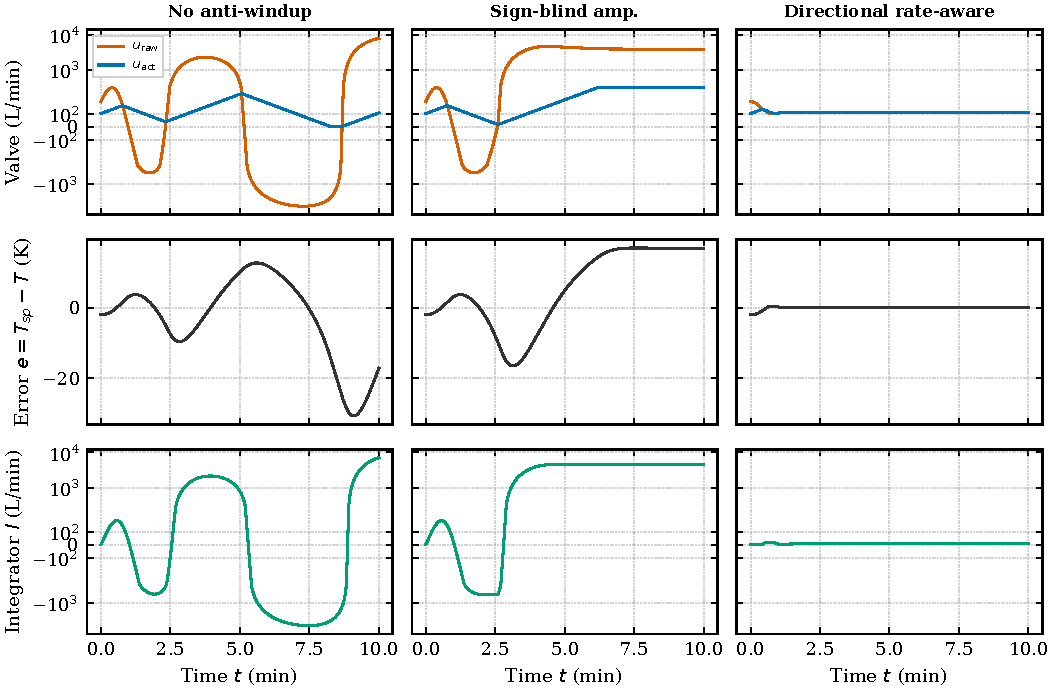
\includegraphics[width=0.92\textwidth]{figures/fig_mechanism.pdf}
    \caption{ZN on the $-2$~K step under three integrator policies: command $u_{\text{raw}}$ and valve position $u_{\text{act}}$ (top), error (middle) and integrator state (bottom); symmetric logarithmic axes.}
    \label{fig:mechanism}
\end{figure*}

\paragraph{Factorial reading: the trigger, not the sign, restores the loop.} On the nominal step the amplitude-only variants avoid the latch but still integrate through the rate-limited moves (IAE $\vZNamp$ and $\vCCamp$~K$\cdot$min for ZN and CC), whereas the rate-aware variants recover the tracking ($\vZNrateunc$ and $\vCCrateunc$ with the unconditional freeze, $\vZNdir$ and $\vCCdir$ with the directional one). For TL, AMIGO, SIMC and Optimal ITAE the amplitude limit is never reached on this step, so the amplitude-triggered variants coincide with no anti-windup. Sign awareness is second order once the trigger is rate-aware. The conclusion does not depend on the step (Table~\suppref{tab:antiwindup_scenarios}): on the $\pm 5$~K steps the amplitude-only variants leave ZN, CC, AMIGO and Optimal ITAE at IAE between $\vscenampmin$ and $\vscenampmax$~K$\cdot$min, against $\vscendirmin$ to $\vscendirmax$ with the rate-aware directional rule, so loops whose nominal step does not expose the problem are also affected by large moves. Sign-blind clamping remains worse than no anti-windup for the empirical rules on the $-5$~K step and on the load profile.


\subsection{Back-calculation and its tracking constant}
\label{subsec:backcalc}
Supplementary Fig.~\suppref{fig:tt_curve} scans $T_t$ from $0.525\,\Delta t$ to $10\,T_i$ for the three steps. The physical range of the tracking constant is $T_d \le T_t \le T_i$; below $\Delta t$ the explicit Euler step of Eq.~\eqref{eq:back_calculation}, which multiplies $I$ by $1 - \Delta t/T_t$, over-corrects, and below $\Delta t/2$ it diverges. Both limits come from that discretization: with the exact factor $1 - e^{-\Delta t/T_t}$ (or an implicit step) they do not exist (ZN at $\Delta t/T_t = \vexZNratio$: IAE $\vexZNeuler$ with Euler, $\vexZNexact$ exact; Table~\suppref{tab:exact_backcalc}). A fair comparison needs one $T_t$ per loop rather than the best $T_t$ per step. The main criterion is the one a designer can apply without the directional rule: $T_t^{\mathrm{sel}}$ is chosen inside $[T_d, T_i]$ on the $-2$~K design step and judged on the $\pm 5$~K steps (Table~\ref{tab:antiwindup_tt_summary}). Its worst IAE ratio to the directional rule on $\pm 5$~K lies between $\vttcvmin$ and $\vttcvmax$ over the six loops: back-calculation with one constant chosen on the design step matches the directional rule on larger steps. A second criterion, $T_t^{\mathrm{mm}}$, minimizes the largest ratio over the three steps and gives $\vttmmmin$ to $\vttmmmax$; it is in-sample and uses the directional rule as reference, so it only confirms the first. Three of these choices are boundary solutions: for \vttcvlower{} $T_t^{\mathrm{sel}}$ sits on the lower edge, $T_t = T_d$, and for \vttcvupper{} on the upper edge, $T_t = T_i$. Without the restriction the minimum leaves the range: to $\Delta t$ for ZN and CC and to the largest value scanned, $\vttfreeSIMCovTi\,T_i$, for SIMC (Supplementary Fig.~\suppref{fig:tt_curve}). With the exact tracking factor the ZN and CC minima move to the smallest value scanned ($\vttfreexZN$ and $\vttfreexCC$~min, Table~\ref{tab:antiwindup_tt_summary}): their IAE keeps falling as the tracking strengthens, so the edge $T_d$ binds and the Euler minimum at $\Delta t$ is a discretization artefact. Leaving the range changes the worst ratio on $\pm 5$~K by up to $\vttfreediffmax$, for \vttfreediffloop{}, where it gets worse, and by at most $\vttfreediffrest$ for the other loops (Table~\ref{tab:antiwindup_tt_summary}): the physical range costs nothing out of sample, but it does not make these choices interior. For SIMC the criterion chooses little or no back-calculation: $T_t^{\mathrm{sel}} = T_i$, the weakest tracking in the range, gives $\vSIMCcvtwo$, $\vSIMCcvm$ and $\vSIMCcvp$~K$\cdot$min on $-2$, $-5$ and $+5$~K, close to no anti-windup ($\vSIMCnone$, $\vSIMCfivemnone$, $\vSIMCfivepnone$) and better than the directional rule ($\vSIMCdir$, $\vSIMCfivemdir$, $\vSIMCfivepdir$). The usual defaults are worse, with worst ratios up to $\vttsqrtmax$ for $T_t = \sqrt{T_iT_d}$ and $\vtttimax$ for $T_t = T_i$, the value associated with conditioning techniques \cite{peng1996nonlinear}. The comparison is not limited to the IAE (Table~\suppref{tab:antiwindup_tt_tvmp}). Only for ZN and CC, over the three steps, does back-calculation with $T_t^{\mathrm{sel}}$ move the valve less ($\vempTVlower$ of $\vempcases$ cases) and overshoot less ($\vempMplower$ of $\vempcases$; CC on $+5$~K: travel $\vCCfiveTVbc$ against $\vCCfiveTVdir$~L/min with the directional rule, overshoot $\vCCfiveMpbc\%$ against $\vCCfiveMpdir\%$). For TL, SIMC and Optimal ITAE it moves the valve more in $\vrestTVhigher$ of $\vrestcases$ cases and overshoots more in $\vrestMphigher$ and less in none (SIMC on $-5$~K: travel $\vSIMCfiveTVbc$ against $\vSIMCfiveTVdir$~L/min; Optimal ITAE on $+5$~K: overshoot $\vOPTfiveMpbc\%$ against $\vOPTfiveMpdir\%$). The advantage of the directional rule is therefore that it needs no per-loop constant, not that it performs better; its behaviour depends on the slew limit and on $\Delta t$ through $u_{\text{act}}$, which the next subsection maps.



\begin{table*}[t]
\centering
\footnotesize
\caption{One tracking constant per loop. $T_t^{\mathrm{mm}}$ minimizes, over the physical range $[T_d, T_i]$, the largest IAE ratio (back-calculation over the directional rule, Eq.~\eqref{eq:clamping_antiwindup}) across the $-2$, $-5$ and $+5$~K steps; $T_t^{\mathrm{cv}}$ is chosen on the $-2$~K design step only and judged on $\pm 5$~K. Entries are the worst ratio over the steps (values above $1$: back-calculation is worse).}
\label{tab:antiwindup_tt_summary}
\resizebox{\ifdim\width>\textwidth\textwidth\else\width\fi}{!}{%
\begin{tabular}{lccccccc}
\toprule
Method & \([T_d, T_i]\) (min) & $T_t^{\mathrm{mm}}$ (min) & worst ratio, $T_t^{\mathrm{mm}}$ & worst ratio, $\sqrt{T_iT_d}$ & worst ratio, $T_t=T_i$ & $T_t^{\mathrm{cv}}$ (min) & worst ratio on $\pm 5$~K, $T_t^{\mathrm{cv}}$ \\
\midrule
Ziegler-Nichols & [0.047, 0.187] & 0.047 & 1.02 & 1.09 & 1.97 & 0.047 & 1.02 \\
Cohen-Coon & [0.033, 0.217] & 0.033 & 0.94 & 0.98 & 1.90 & 0.033 & 0.94 \\
Tyreus-Luyben & [0.056, 0.779] & 0.554 & 0.94 & 1.37 & 1.01 & 0.554 & 0.94 \\
AMIGO & [0.045, 0.327] & 0.139 & 1.00 & 1.00 & 1.26 & 0.121 & 1.00 \\
Skogestad SIMC & [0.031, 0.643] & 0.643 & 0.90 & 1.15 & 0.90 & 0.643 & 0.86 \\
Optimal ITAE ($M_s^{\mathrm{FOPTD}} \leq 1.6$) & [0.032, 0.465] & 0.300 & 1.01 & 1.20 & 1.18 & 0.300 & 0.98 \\
\bottomrule
\end{tabular}%
}
\end{table*}



\subsection{Regime map: where the slew-rate trigger matters}
\label{subsec:regime}
Supplementary Fig.~\suppref{fig:smax_map} and Table~\suppref{tab:smax_map} (first row of each loop) repeat the $-2$~K step for slew limits from $20$ to $320$~L/min$^2$ with the gains fixed. The ratio of amplitude-only to rate-aware directional clamping, $R = \mathrm{IAE}_{\mathrm{amp}}/\allowbreak\mathrm{IAE}_{\mathrm{rate}}$, measures what the rate trigger buys ($R > 1$: it helps). For ZN and CC it is $\vmapCCmin$ to $\vmapZNmax$ at every limit, because the amplitude limit is reached and the integrator winds up during the rate-limited ramp. Sign-blind clamping latches the valve at the upper stop for $S_{\max} \ge \vlatchfromZN$~L/min$^2$, with one exception: for ZN at $240$~L/min$^2$ the same mechanism latches it at the lower stop (closed for $\vsbZNlowtime$~min), the mirror case of Proposition~\ref{prop:latch}, and the reactor heats to $\vsbZNlowerr$~K at $t_f$, still rising (Supplementary Section~\suppref{supp:aw}). For AMIGO $R$ is $\vmapAMIGOtwenty$ at $20$~L/min$^2$, $\vmapAMIGOeighty$ at the benchmark value and $\vmapAMIGOlast$ at $320$, and for Optimal ITAE $\vmapOptimalITAEtwenty$, $\vmapOptimalITAEeighty$ and $\vmapOptimalITAElast$: the trigger matters when the valve is slow compared with what the loop demands. For TL $R$ stays between $\vmapTLmin$ and $\vmapTLmax$. Re-optimizing the Optimal ITAE gains at each limit gives $R$ from $\vretunedfirst$ to $\vretunedlast$ (Table~\suppref{tab:smax_retuned}), so the map is not an artefact of gains designed at $80$~L/min$^2$.

\paragraph{SIMC is a counterexample.} For SIMC the rate-aware trigger makes the loop \emph{worse} than no anti-windup: $R$ is $\vSIMCratioff$, $\vSIMCratioeighty$ and $\vSIMCratiolast$ at $45$, $80$ and $320$~L/min$^2$ (it exceeds $1$ only at $20$, $\vSIMCratiotwenty$), and the IAE is $\vSIMCdir$ against $\vSIMCnone$~K$\cdot$min on the $-2$~K step, $\vSIMCfivemdir$ against $\vSIMCfivemnone$ on $-5$~K and $\vSIMCfivepdir$ against $\vSIMCfivepnone$ on $+5$~K, and likewise with a deadband and at a second operating point (Table~\ref{tab:robustness_ext}). The slow, well-damped loop asks for valve moves only slightly faster than the slew limit and only briefly ($\vTrlSIMC$~min slew-limited on the $-2$~K step, against $\vTrlothersmin$ to $\vTrlothersmax$~min for the other loops), so little windup accumulates; freezing the integrator during those samples removes integral action the loop needed, and the freeze acts as a delay rather than as a protection. Table~\suppref{tab:rate_demand} relates the outcome to the rate demand $\rho = \max_k|u_k - u_{k-1}|/(S_{\max}\Delta t)$ of the same loop with the slew limit removed (setpoint kick excluded), which uses the IAE of neither rule and can be computed from one simulation before the rule is chosen. On the $\vncases$ nominal cases from which the rule below is drawn (six loops, three steps, nine limits), the trigger improved $\vnrhohihelp$ of the $\vnrhohi$ cases with $\rho \ge 1$; with $\rho < 1$, $R$ ranged from $\vrholoratiomin$ to $\vrholoratiomax$, and $\rho$ does not separate SIMC from the other loops (\vrhohelplowloop{} gains with $\rho = \vrhohelplow$). On conditions not used to draw it (second operating point and deadbands, Table~\suppref{tab:rate_demand_check}) all $\vchkrhohihelp$ loop--condition pairs with $\rho \ge 1$, from $\vchkhiloops$ loops (\vchkhilooplist{}), improved; only $\vchknear$ of them lie near the threshold (\vchknearlist{}). Under sensor noise of $0.05$~K, $\rho$ computed on the raw command measures the noise ($\rho$ up to $\vrhonzrawSIMCmax$ for SIMC, $\vrhonzrawwrong$ of $\vrhonzcases$ cases misclassified), whereas on the command of a loop with the measurement filter ($\tau_m = 0.05$~min) it separates the cases as without noise ($\vrhonzfiltwrong$ misclassified; Table~\suppref{tab:rho_noise}). We offer $\rho \ge 1$ as a heuristic, not a validated criterion, calibrated on this noise-free reactor model, which does not transfer as is to the second plant of Section~\ref{subsec:hx}: switch the rate-aware trigger on when the loop demands faster valve moves than the slew limit allows, and check its effect otherwise.




\subsection{Actuator model, implementation and operating points}
\label{subsec:robustness_ext}
Table~\ref{tab:robustness_ext} repeats the comparison under the changes of the two groups of Section~\ref{sec:intro} and at a second operating point; Table~\ref{tab:conclusion_robustness} collects, for every conclusion, the conditions under which it was tested.

\subsubsection{Actuator model: deadband and stiction}
\label{subsubsec:actuator_model}
\emph{Does the verdict survive a valve that does not follow the controller's copy of the limits?} These are properties of the actuator, not choices of the controller. A valve deadband of $6$~L/min is modelled as a backlash operator applied after the amplitude and slew limits (Eq.~\suppref{eq:backlash}), so that $u_{\text{act}}$, which the anti-windup logic uses, includes the slew limit but not the backlash. The deadband raises every IAE, but the ordering persists: sign-blind clamping still latches ZN and CC, and amplitude-only clamping leaves them at least $\vdbampratiomin$ times worse than the rate-aware rule, which stays within $\vdbsixworstpct\%$ of back-calculation with $T_t = \sqrt{T_iT_d}$ for every loop but is up to $\vdbsixworstpctcv\%$ worse than back-calculation with $T_t^{\mathrm{sel}}$ (Table~\suppref{tab:antiwindup_deadband}). Where the backlash sits also matters: placed before the slew limit, with the controller's $u_{\text{act}}$ unchanged, it changes the IAE by up to $\vorderTwodIAE\%$ and the order of loops and of policies (Table~\suppref{tab:order_variants}). Valve stiction (two-parameter model \cite{choudhury2005modelling} after the slew limit, moderate and severe; Table~\suppref{tab:stiction}) makes the loop hunt in $\vstickmoderatehunt\%$ and $\vstickseverehunt\%$ of the runs with the working policies, which no integrator policy prevents; the latch and the amplitude-only windup remain (at least $\vsticksbmin$ and $\vstickampmin$ times the IAE of the rate rule for ZN and CC), but back-calculation against the rate rule becomes erratic ($\vstickbcmin$ to $\vstickbcmax$) and the SIMC counterexample depends on the step ($\vstickSIMCmin$ to $\vstickSIMCmax$). In short, the latch and the value of the slew-rate trigger survive these defects, whereas the comparison of back-calculation with the directional rule depends on how the actuator is specified.

\subsubsection{Order of evaluation and discretization}
\label{subsubsec:order}
\emph{Do choices inside the controller that comparisons rarely state change the verdict?} Table~\suppref{tab:order_variants} changes one choice at a time. Applying the slew limit before the saturation changes no ranking (IAE within $\vorderOnedIAE\%$). Feeding the derivative with the unfiltered measurement under noise changes the IAE by up to $\vorderThreeNoisydIAE\%$, and discretizing the measurement filter by explicit Euler by up to $\vorderFourdIAE\%$ without noise. With $\Delta t/\tau_m = 0.4$ the explicit Euler filter is a poor discretization, so a difference of this size is an expected warning, not a finding; it is reported because such a filter is easily coded and seldom stated. Over the four variants, of the $\vdtwopolflips$ policy swaps, $\vdtwoworkflips$ are between the rate rule and the two back-calculations; sign-blind and amplitude-only clamping stay at least $\vdtwosbmin$ and $\vdtwoampmin$ times worse than the rate rule for ZN and CC in every variant. In short, the order of the two limits is immaterial here, whereas the discretization of the measurement path can reorder close competitors without reversing the main conclusions.

\subsubsection{Operating points}
\label{subsubsec:op_points}
\emph{Is the verdict specific to the nominal operating point?} At a second operating point, $q_{j,ss} = 150$~L/min, with the FOPTD re-identified and the analytical rules re-tuned (Table~\suppref{tab:antiwindup_second_op}), sign-blind clamping is again worse than no anti-windup for ZN and CC, and the rate-aware rule recovers $\vopZNdir$ and $\vopCCdir$ against $\vopZNamp$ and $\vopCCamp$ with amplitude-only clamping; AMIGO needs the rate-aware trigger ($\vopAMIGOnone$ without, $\vopAMIGOdir$ with), SIMC does not ($\vopSIMCnone$ without, $\vopSIMCdir$ with). A third point chosen by a declared criterion is in Table~\suppref{tab:c2_ablation}. In short, the ordering of the policies holds at the operating points tested, all of which belong to one reactor model.

\begin{table*}[t]
\centering
\footnotesize
\setlength{\tabcolsep}{3pt}
\caption{IAE (K$\cdot$min) of five integrator policies with a valve deadband of $6$~L/min and at a second operating point $q_{j,ss} = 150$~L/min with re-identified FOPTD and re-tuned analytical rules (the optimal tuning was not re-optimized there); valve $[0, 300]$~L/min, $S_{\max} = 80$~L/min$^2$. SB: sign-blind amplitude clamping; Amp.: amplitude-only directional; Rate: amplitude-plus-rate directional (Eq.~\eqref{eq:clamping_antiwindup}); BC: back-calculation with $T_t = \sqrt{T_iT_d}$; BC$^{\mathrm{cv}}$: with the $T_t^{\mathrm{cv}}$ of Table~\ref{tab:antiwindup_tt_summary}, re-chosen by the same criterion at the second point.}
\label{tab:robustness_ext}
\begin{tabular}{lcccccccccc}
\toprule
 & \multicolumn{5}{c}{Deadband $6$~L/min} & \multicolumn{5}{c}{$q_{j,ss} = 150$~L/min} \\
Tuning & SB & Amp. & Rate & BC & BC$^{\mathrm{cv}}$ & SB & Amp. & Rate & BC & BC$^{\mathrm{cv}}$ \\
\midrule
ZN & 106.99 & 24.82 & 1.65 & 1.83 & 1.63 & 61.48 & 16.13 & 1.00 & 1.06 & 1.00 \\
CC & 104.69 & 23.01 & 1.76 & 1.60 & 1.48 & 59.68 & 15.42 & 1.05 & 0.99 & 0.96 \\
TL & 1.50 & 1.50 & 1.06 & 1.40 & 1.02 & 1.41 & 1.41 & 1.20 & 1.56 & 0.97 \\
AMIGO & 2.71 & 2.71 & 1.54 & 1.54 & 1.54 & 2.16 & 2.16 & 1.07 & 1.07 & 1.07 \\
SIMC & 1.55 & 1.55 & 1.92 & 1.75 & 1.67 & 1.16 & 1.16 & 1.42 & 1.56 & 1.25 \\
Optimal ITAE & 2.58 & 2.58 & 1.23 & 1.22 & 1.26 & -- & -- & -- & -- & -- \\
\bottomrule
\end{tabular}
\end{table*}


\subsection{A second plant}
\label{subsec:hx}
The study was repeated on a heat exchanger built for this purpose, not a published benchmark: a well-mixed shell and a tube of two cells in series, cooled by the same valve, without reaction kinetics, reverse-acting, open-loop stable (slowest eigenvalue $\vhxeigslow$~min$^{-1}$) and with a $0.20$~min transport delay on the outlet (Supplementary Section~\suppref{supp:hx}). Its identified FOPTD has $K = \vhxK$~K/(L/min) and a measured $\theta/\tau = \vhxr$; the six loops were tuned by the same rules and the Optimal ITAE was re-optimized on it (Table~\ref{tab:hx}). The results are consistent with the mechanism for the empirical rules and differ elsewhere. For ZN and CC amplitude-only clamping is at least $\vhxampratemin$ times worse than the rate-aware rule on the $\pm 5$~K steps, as on the reactor. Sign-blind clamping is $\vhxsbnonemin$ to $\vhxsbnonemax$ times worse than no anti-windup, but the valve never rests at the upper stop: these loops wind up through the slew limit into a sustained oscillation, the hypotheses of Proposition~\ref{prop:latch} are not reached and there is no latch. The rate-aware trigger makes TL worse on every step ($\vhxTLratemin$ to $\vhxTLratemax$ times the IAE without anti-windup) although its $\rho$ reaches $\vhxbadrhomax$; on this plant $\rho \ge 1$ was followed by an improvement in only $\vhxnrhohihelp$ of $\vhxnrhohi$ cases (exceptions: \vhxbadloops{}), so the heuristic does not transfer as is. Back-calculation with $T_t^{\mathrm{sel}}$ gives $\vhxbcmin$ to $\vhxbcmax$ times the IAE of the rate-aware rule.

\begin{table*}[t]
\centering
\footnotesize
\setlength{\tabcolsep}{3pt}
\caption{Second plant: the heat exchanger described in Supplementary Section~\suppref{supp:hx}: IAE (K$\cdot$min) of the integrator policies on the $-5$~K step (first five columns) and of no anti-windup and the rate-aware rule on the $-2$~K step (last two); same valve ($[0, 300]$~L/min, $S_{\max} = 80$~L/min$^2$), loops tuned by the same rules, Optimal ITAE re-optimized, BC$^{\mathrm{sel}}$ with $T_t^{\mathrm{sel}}$ chosen on this plant.}
\label{tab:hx}
\begin{tabular}{lccccccc}
\toprule
 & \multicolumn{5}{c}{$-5$~K step} & \multicolumn{2}{c}{$-2$~K step} \\
Tuning & None & SB & Amp. & Rate & BC$^{\mathrm{sel}}$ & None & Rate \\
\midrule
ZN & 49.49 & 50.99 & 38.78 & 3.77 & 3.79 & 2.15 & 1.15 \\
CC & 54.98 & 60.58 & 37.96 & 3.69 & 3.68 & 4.73 & 1.09 \\
TL & 3.83 & 3.83 & 3.83 & 6.19 & 5.33 & 1.45 & 1.96 \\
AMIGO & 5.65 & 5.65 & 5.65 & 4.24 & 4.25 & 1.56 & 1.42 \\
SIMC & 4.31 & 4.31 & 4.31 & 4.74 & 4.26 & 1.42 & 1.51 \\
Optimal ITAE & 5.22 & 5.22 & 5.22 & 4.12 & 3.95 & 1.37 & 1.16 \\
\bottomrule
\end{tabular}
\end{table*}


\subsection{Measurement path}
\label{subsec:measurement_path}
The noise vulnerability of the empirical rules is often attributed to a high sensitivity peak, which on the identified FOPTD is $\vMsFZN$ for ZN and $\vMsFCC$ for CC. On the exact linearization the peaks are only $\vSlinZN$ and $\vSlinCC$ (Table~\ref{tab:testbed}); the FOPTD values largely reflect its apparent delay. What separates the loops is the gain from measurement noise to the valve command, $CS = C/(1+L)$: at high frequency $CS \to C$, so its peak is the plateau of the filtered PID, $|K_p|(1+N)$, which is $\vCSZN$ and $\vCSCC$~(L/min)/K for ZN and CC against $\vCSSIMC$ for SIMC. A first-order measurement filter ($\tau_m = 0.05$~min) lowers the valve travel at a noise level of $\sigma = 0.01$~K by a factor of $\vfiltfactmin$ to $\vfiltfactmax$, and lowering the derivative-filter coefficient from $N = 10$ to $N = 3$ cuts $|K_p|(1+N)$ of ZN and CC by $\vNcut\%$ without changing their noise-free error (Supplementary Tables~\suppref{tab:noise_sensitivity}--\suppref{tab:n_design}, $30$ noise realizations per case). Noise also qualifies the comparison of Section~\ref{subsec:backcalc} (Table~\suppref{tab:noise_policies}, $30$ realizations): at $\sigma = 0.05$~K back-calculation with the noise-free $T_t^{\mathrm{sel}}$ is up to $\vnzbchimaxpct\%$ worse than the directional rule for \vnzbcworse{} and better for \vnzbcbetter{} (ratios $\vnzbclomin$ to $\vnzbclomax$ at $0.01$~K), whereas no anti-windup stays at least $\vnzempnonemin$ times worse for ZN and CC and the rule still worsens SIMC ($\vnzSIMCdir$ against $\vnzSIMCnone$). The mechanism is the tracking term, not more frequent saturation: noise keeps a limit cutting the command in the same share of samples under both rules (at least $\vmechcutmin$ for ZN and CC), but with $T_t = T_d$ the term $(\Delta t/T_t)(u_{\text{act}} - u_{\text{raw}})$ feeds $\vmechtrackmin$ to $\vmechtrackmax$~L/min per sample into the integrator, whose deviation from its noise-free path is $\vmechrmsratiomin$ to $\vmechrmsratiomax$ times that of the directional rule (Table~\suppref{tab:noise_mechanism}). Re-choosing $T_t$ under noise moves it up for \vnzttchanged{} and narrows the gap without closing it (worst ratio on $-2$~K from $\vnzttbeforemax$ to $\vnzttaftermax$; Table~\suppref{tab:noise_ttcv}), while the measurement filter brings the worst ratio over the three steps from $\vextrawmax$ to $\vextfiltmax$ (Table~\suppref{tab:noise_policies_ext}). The equivalence of Section~\ref{subsec:backcalc} is a noise-free result, and the measurement path is part of the implementation that a comparison must state.

\subsection{Robustness of the conclusions and practical recommendations}
\label{subsec:robustness_summary}
Table~\ref{tab:conclusion_robustness} reads the results above conclusion by conclusion. In every reactor condition tested sign-blind clamping stays far worse than the rate-aware rule for the high-gain loops (the latch itself was checked only where marked) and the slew-rate trigger keeps its role; the equivalence of back-calculation and the directional rule is the most fragile conclusion, lost with sensor noise and under stiction; the heuristic $\rho \ge 1$ holds only on the reactor, on a filtered or noise-free loop, and with one exception at $250$~L/min. For a practitioner this means: on a reverse-acting loop, implement conditional integration in the product form of Eq.~\eqref{eq:clamping_antiwindup} and never copy the direct-acting condition; switch the slew-rate trigger on when the loop demands faster moves than the valve allows, and check it on slow, well-damped loops, where it can delay integral action; without sensor noise either the directional rule or back-calculation with a constant chosen on the design step will do, whereas with noise the directional rule, or a filtered measurement, is the safer choice; under stiction expect hunting with every integrator policy and do not trust a ranking of back-calculation against the rule; with a measured valve position use a detection band. In every case, state the order of the limits, the discretization of the filters and the actuator model.

% Qualitative summary written from existing tables only; it carries no result number.
\begin{table*}[t]
\centering
\footnotesize
\setlength{\tabcolsep}{3pt}
\caption{Robustness of the conclusions: for each conclusion and condition, whether it holds, holds in part, fails or was not tested, with the table or section that supports the entry (T: main text; S: Supplementary). Filled only from results reported in this paper; ``not tested'' means that no run addressed the conclusion under that condition. Measured position: anti-windup fed with a measured valve position (Section~\ref{subsec:limitations}). Other points: $q_{j,ss} = 150$ and $250$~L/min.}
\label{tab:conclusion_robustness}
\begin{tabular}{@{}>{\raggedright\arraybackslash}p{3.5cm}*{7}{>{\raggedright\arraybackslash}p{1.72cm}}@{}}
\toprule
Conclusion & CSTR nominal & Meas.\ noise & Deadband & Stiction & Measured position & Other CSTR points & Heat exchanger \\
\midrule
Sign-blind clamping latches the loop at full cooling & holds (T\ref{tab:antiwindup_ablation}, \suppref{tab:antiwindup_mechanism}) & in part$^a$ (\suppref{tab:order_variants}) & holds (\suppref{tab:antiwindup_deadband}) & holds (\suppref{tab:stiction}) & not tested & in part$^b$ (\suppref{tab:antiwindup_second_op}, \suppref{tab:c2_ablation}) & fails$^c$ (\S\ref{subsec:hx}, \suppref{tab:hx_ablation}) \\
The slew-rate trigger, not sign awareness, restores the high-gain loops & holds (T\ref{tab:antiwindup_ablation}) & in part$^d$ (\suppref{tab:order_variants}) & holds (\suppref{tab:antiwindup_deadband}) & holds (\suppref{tab:stiction}) & not tested & holds (\suppref{tab:antiwindup_second_op}, \suppref{tab:c2_ablation}) & holds (T\ref{tab:hx}) \\
The trigger is not universally beneficial (SIMC; TL on the exchanger) & holds (T\ref{tab:antiwindup_ablation}, \S\ref{subsec:regime}) & holds (\suppref{tab:noise_policies}) & holds (T\ref{tab:robustness_ext}) & in part$^e$ (\suppref{tab:stiction}) & not tested & holds (\suppref{tab:antiwindup_second_op}, \suppref{tab:c2_ablation}) & holds (T\ref{tab:hx}) \\
Back-calculation with $T_t^{\mathrm{sel}}$ matches the directional rule without noise, not with it & holds (T\ref{tab:antiwindup_tt_summary}) & holds: gap$^f$ (\suppref{tab:noise_policies}--\suppref{tab:noise_policies_ext}) & holds (\suppref{tab:antiwindup_deadband}) & fails$^g$ (\suppref{tab:stiction}) & in part$^h$ (\suppref{tab:measured_position}) & holds (\suppref{tab:antiwindup_second_op}, \suppref{tab:c2_ablation}) & holds (T\ref{tab:hx}) \\
Heuristic $\rho \ge 1$ for switching the trigger on & holds (\suppref{tab:rate_demand}) & in part$^i$ (\suppref{tab:rho_noise}) & holds (\suppref{tab:rate_demand_check}) & not tested & not tested & in part$^j$ (\suppref{tab:rate_demand_check}, \suppref{tab:c2_ablation}) & fails (\S\ref{subsec:hx}, \suppref{tab:hx_smax_map}) \\
Order of the limits and discretization matter selectively & holds (\suppref{tab:order_variants}) & holds (\suppref{tab:order_variants}) & holds$^k$ (\suppref{tab:order_variants}) & not tested & not tested & not tested & not tested \\
\bottomrule
\end{tabular}

\vspace{2pt}
\parbox{\textwidth}{\scriptsize $^a$ Sign-blind clamping stays far worse than the rate rule for ZN and CC in the noisy variants; the latch itself was not checked under noise. $^b$ Worse than no anti-windup for ZN and CC at $150$~L/min and on two of the three steps at $250$~L/min; the latch was not checked there, and at $250$~L/min the $-5$~K step saturates every policy. $^c$ No latch: the hypotheses of Proposition~\ref{prop:latch} are not reached. $^d$ Amplitude-only clamping stays worse than the rate rule for ZN and CC; the factorial of sign awareness was not repeated under noise. $^e$ The SIMC result depends on the step. $^f$ The equivalence is a noise-free result; with noise back-calculation is worse for the high-gain loops, and filtering narrows the gap. $^g$ The ratio to the rate rule becomes erratic. $^h$ Back-calculation with the measured position is worse than the rule with the detection band in some loop--step pairs. $^i$ Misclassifies cases on the raw measurement, not on the filtered one. $^j$ Holds at $150$~L/min; fails for TL on $-2$~K at $250$~L/min. $^k$ Backlash before the slew limit, variant (ii).}
\end{table*}


\subsection{Limitations}
\label{subsec:limitations}
The study uses one reactor model with constant physical properties and simulates deadband and stiction only for the anti-windup policies, and deterministic responses in the main text; under sensor noise only the three main policies were compared (Table~\suppref{tab:noise_policies}), and the back-calculation constants were chosen without noise. The controller is assumed to know $u_{\text{act}}$, i.e.\ the slew limiter is replicated at its output. Feeding Eq.~\eqref{eq:clamping_antiwindup} with a measured position (lag $0.01$~min, noise $0.3$~L/min) instead freezes the integrator in $\vposspurmin$ to $\vposspurmax\%$ of the samples in which no limit acts and raises the IAE by up to $\vposworstpct\%$ (\vposworstloop{}); a detection band $\varepsilon_u = 3\sigma_v + S_{\max}\tau_v$ removes most of these freezes (at most $\vposspurbandmax\%$, IAE within $\vposbandpct\%$), and back-calculation with the measured position loses at most $\vposbcpct\%$ (Table~\suppref{tab:measured_position}). A second plant, a heat exchanger built for this study, was tested (Section~\ref{subsec:hx}); it supports the role of the slew-rate trigger for the high-gain loops but not the transfer of the $\rho$ heuristic or of the latch, and no higher-fidelity plant was tested. The regime map, the back-calculation constants and the loop-by-loop numbers refer to the plants and valve studied. Dynamic anti-windup compensators were not compared. The six test-bed loops are fixed-gain PID controllers; gain scheduling and model-based controllers are outside the scope.
